\section{Results}

 Performance parameters of the aircraft throughout the mission are listed on Table \ref{tab:results}. The final designed flight path begins with the GO1 accelerating the aircraft to Mach 5.5 and an altitude of 25.33 km. At that point the engines will ignite and initiate a 62.5 s acceleration period until the cruising Mach number of 6.5 is reached where it will maintain speed for 45 seconds. The combined acceleration and cruising phases produce a range of 197.15 km for this mission. The thrust and specific impulse were calculated for the duration of the mission and plotted on Figure \ref{fig:thrustIsp}. During the acceleration portion of the flight the equivalence ratio is highest in order to produce maximum thrust, leading to steadily increasing specific impulse. Once the aircraft reaches the cruising Mach number, the equivalence ratio is lowered so that the thrust can be balanced with the drag, which leads to a sudden drop in Isp. While the calculated mass of 296.3 is slightly above the 273 kg maximum of the GO1 launcher, the mass of the avionics components was taken from the AFRL's GHV release \cite{ghv} and could not be fully designed. In application, the avionics would most likely weigh less, as the mission for the GHV was significantly more complex than this design. A cross section of the vehicle as well as flow conditions during cruising speed are displayed in Figure \ref{fig:totalCrossSection}.

\begin{center}
\begin{tabular}{l c}
\multicolumn{2}{c}{\textbf{Key Performance Parameters}} \\
\hline
Range (km) & 197.15 \\
Starting Mach & 5.5 \\
Cruise Mach & 6.5 \\
Cruise Altitude (km()& 25.33 \\
Acceleration Time (s) & 62.5 \\
Cruise Time (s) & 45 \\
Fuel Weight (kg) & 21 \\
Gross Weight (kg) & 296.3 \\
L/D & 2
\end{tabular}
\captionof{table}{Performance Results}
\label{tab:results}
\end{center}


\begin{figure}[H]
\begin{center}
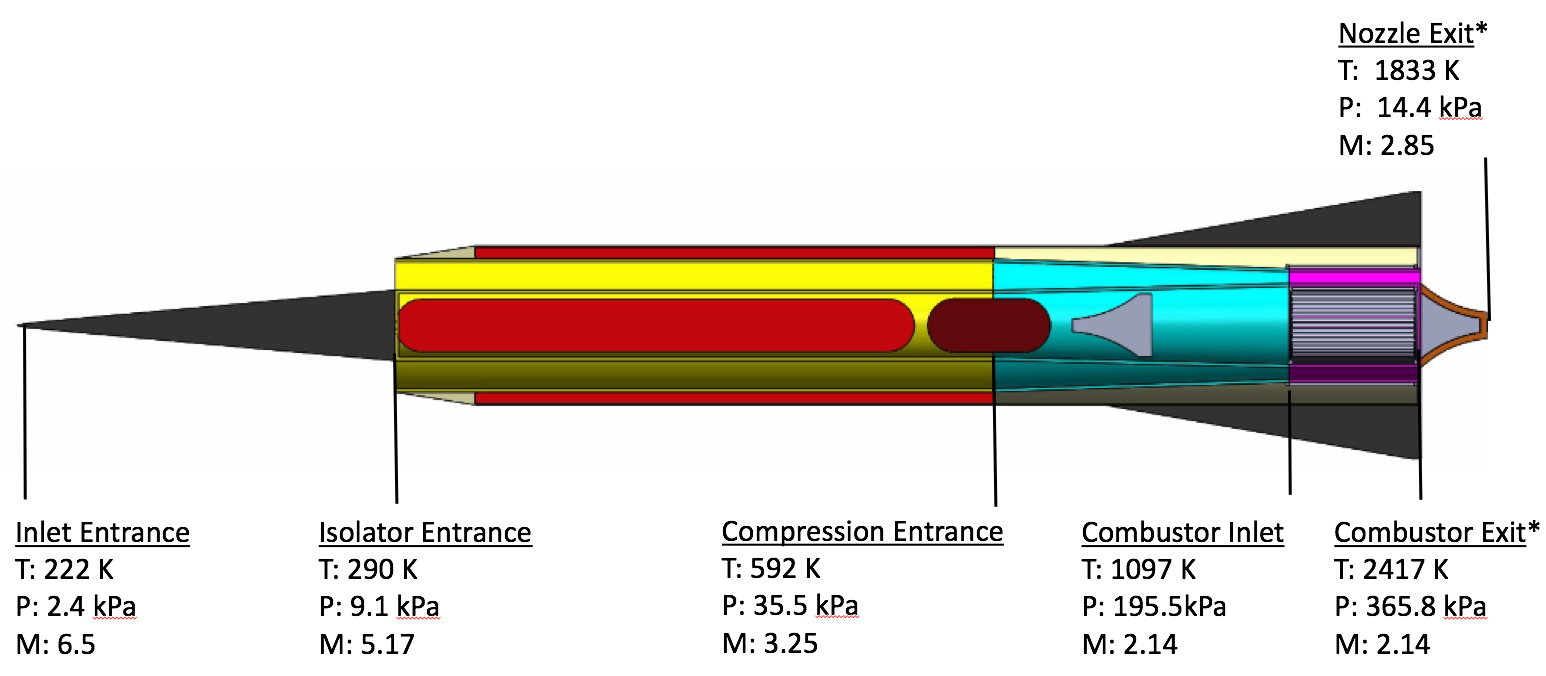
\includegraphics[trim = 0cm 0cm 0cm 1cm, width=\textwidth]{totalCrossSection}
\caption{Flow Station Parameters}
\label{fig:totalCrossSection}
\end{center}
\end{figure}

During cruise, flow will enter the diffusor at Mach 6.5 a static pressure and temperature of 2.4 kPa and 222 K, respectively. The conical diffusor will vary its lateral position such that \ang{5} half angle of the cone will produce an oblique shock that terminates at the cowl lip at the full range of Mach numbers for optimum pressure recovery. The oblique shock slows down the flow to Mach 5.17 and raises static pressure to 9.1 kPa. The flow then travels through an isolator. The isolator was designed to produce a pressure ratio based on the MilStd 5007D \cite{milstd5007D}. Because of the higher combustor inlet Mach numbers RDE’s are capable of operating at, the exit Mach number of the isolator is 3.25 and the static pressure and temperature is 35.5 kPa and 593 K, respectively. The parameters to produce a stable rotating detonation wave within the combustor are highly dependent on the area and entrance pressure of the burner. As a result, a transition is needed to unify the isolator exit and combustor entrance. A compression duct was then added to the design in order to guide the flow to the necessary area as well as raise the static pressure. This isentropic compression raises the static pressure to 195.5 kPa and the static temperature to 1097 K.

\begin{wrapfigure}{r}{0.55\textwidth}
\begin{center}
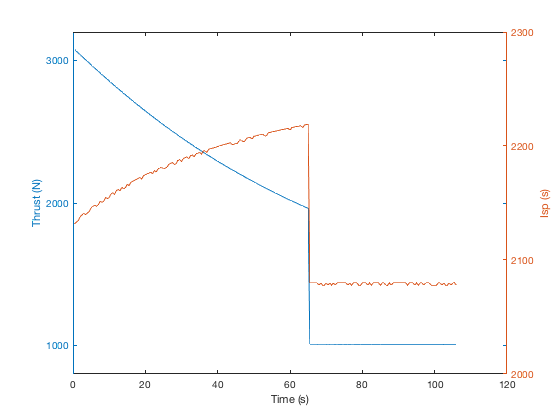
\includegraphics[trim=1cm 1cm 1cm 2cm, width=0.55\textwidth]{thrustIsp}
\caption{Thrust and Isp v. Time}
\label{fig:thrustIsp}
\end{center}
\end{wrapfigure}

        	The ethylene fuel flows from the tanks within the center of the fuselage as well as the exterior of the fuselage through a regenerative heat exchanger that cools the combustor. In order to prevent film boiling in the regenerative heat exchanger, the fuel has to be above supercritical pressure. Consequently, upon injection, the fuel will flash vaporizes. In order to achieve these high pressures, ethylene is stored at 7 MPa, or 40\% above its critical pressure. If there was approximately twice the amount of fuel on the craft, a hydrogen peroxide gas generator and turbopump could be employed to boost low-pressure ethylene above its supercritical conditions. Once the ethylene enters the combustor it mixes with the air flow and enables a rotating detonation wave that leads to an average static pressure of 365.8 kPa and static temperature of 2417 K. The Mach 2.14 flow exiting the combustor then flows through an ablatively cooled aerospike nozzle that expands the gases to 14.4 kPa and a final exit Mach number of 2.85. Figure \ref{fig:thrustIsp} illustrates the vehicle performance over its entire mission.